%This .tex file was written with Heretikz!
%Remember to include \usepackage{tikz-qtree,tikz-qtree-compat}
%java.lang.object
\begin{tikzpicture}
\Tree[.java.lang.object
		[.Tracker
	]
		[.ActivityTracker
				[.TimeTracker
						[.StageGreenTracker
			]
						[.StageRefactorTracker
			]
						[.StageRedTracker
			]
		]
	]
		[.Hint
	]
		[.MasteredExercise
				[.ProfileStats
						[.Profile
			]
		]
	]
		[.Exercise
	]
		[.BasicTimer
	]
		[.ExerciseTests
	]
		[.TaskTimerTests
	]
		[.Error
	]
		[.MasteredExercisesTests
	]
		[.ProfileCollectionTests
	]
		[.BasicTimerTests
	]
		[.TaskTimer
	]
		[.ProfileCollection
	]
		[.HintCollection
	]
]
\end{tikzpicture}
%Stage
\begin{tikzpicture}
\Tree[.Stage
		[.UsefulInfoNotification
	]
]
\end{tikzpicture}
%Application
\begin{tikzpicture}
\Tree[.Application
		[.TDDT
	]
]
\end{tikzpicture}
%EventHandler$\langle$ActionEvent$\rangle$
\begin{tikzpicture}
\Tree[.EventHandler$\langle$ActionEvent$\rangle$
		[.CheckBoxTrollBot
	]
]
\end{tikzpicture}
%TimerTask
\begin{tikzpicture}
\Tree[.TimerTask
		[.TimeUpdateTask
	]
]
\end{tikzpicture}
